\subsection{Key Features Extraction}

Effective deepfake detection relies on the extraction of specific features from videos or images that can reveal inconsistencies or anomalies introduced by the manipulation process. Various techniques are employed to capture these key features, enabling the development of robust detection models. The following are some of the key features commonly extracted for deepfake detection:

\begin{figure}[htbp]
    \centering
    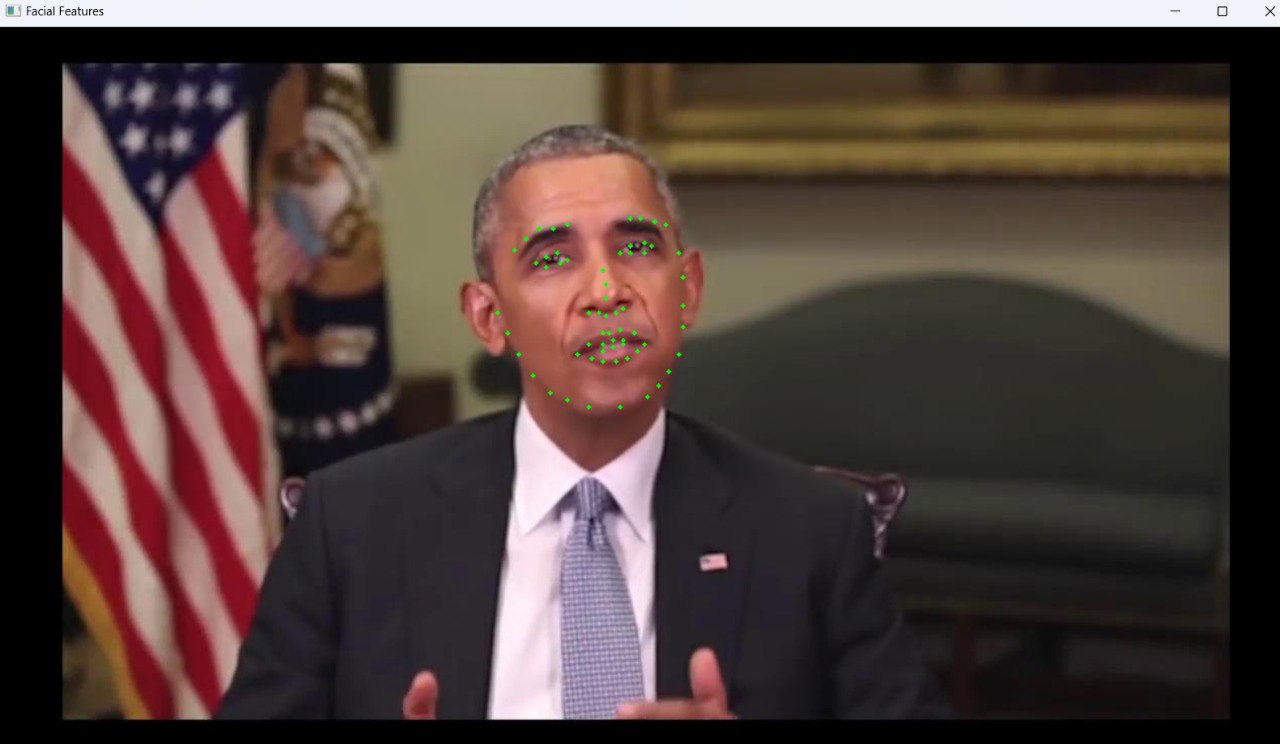
\includegraphics[width= 5in ]{img/featureshighlight.jpg}
    \caption{\textit{Facial landmarks extraction from video}}
\end{figure}
\subsubsection{Abnormal Patterns}

Deepfake detection methods often look for abnormal patterns that deviate from the expected characteristics of genuine content. These patterns can include unnatural facial expressions, inconsistent facial movements. Detecting such abnormalities through pattern recognition can raise suspicion of manipulation.
\begin{figure}[htbp]
    \centering
    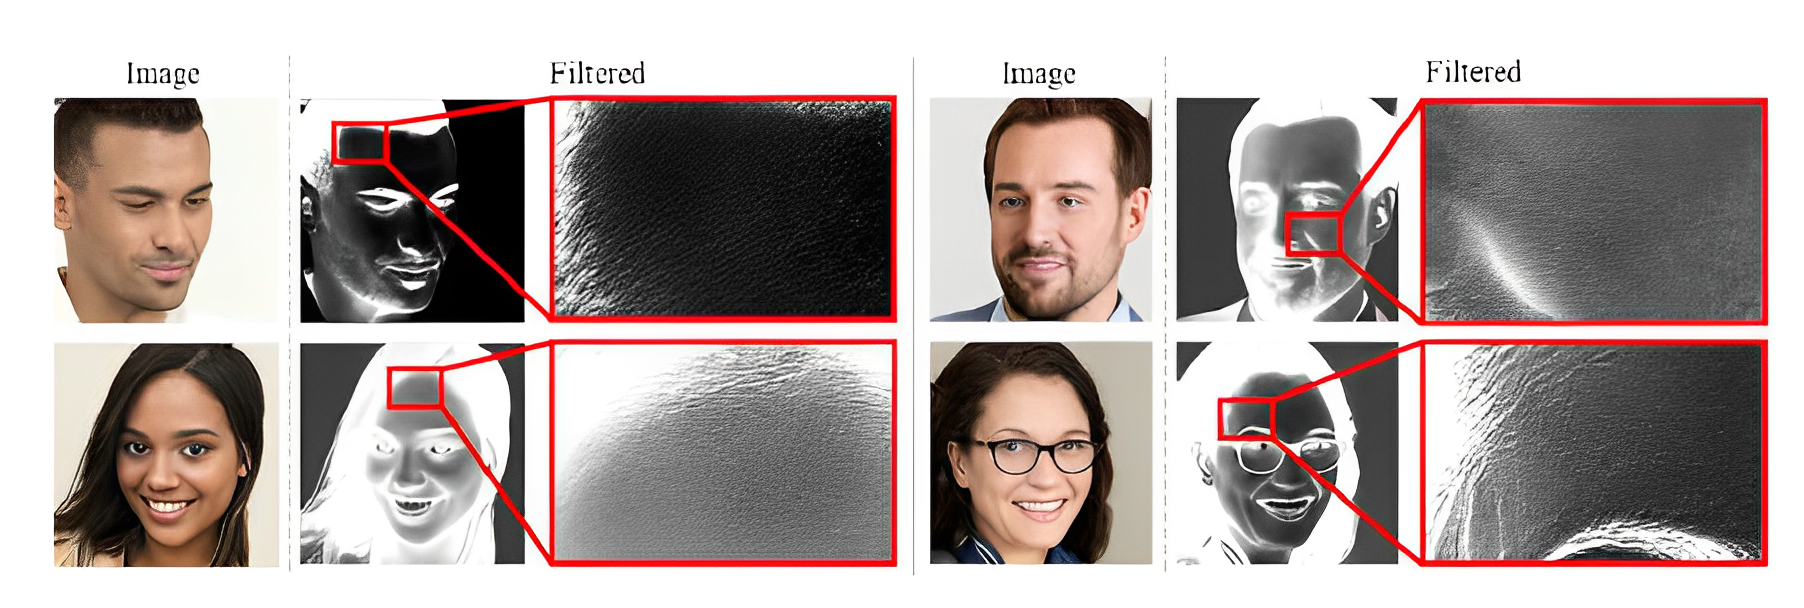
\includegraphics[width=5in]{img/abnormal_pattern.png}
    \caption{\textit{Abnormal Patterns}}
\end{figure}

\subsubsection{Iris Color and Pupil Boundary}

Iris color and pupil boundary analysis involves examining the color distribution and boundary characteristics of the iris and pupil regions. Variances in iris color or irregularities in pupil shape can indicate potential manipulation. Comparing the extracted features of the iris and pupil between frames can help detect abnormal variations introduced by deepfake techniques.
\begin{figure}[htbp]
    \centering
    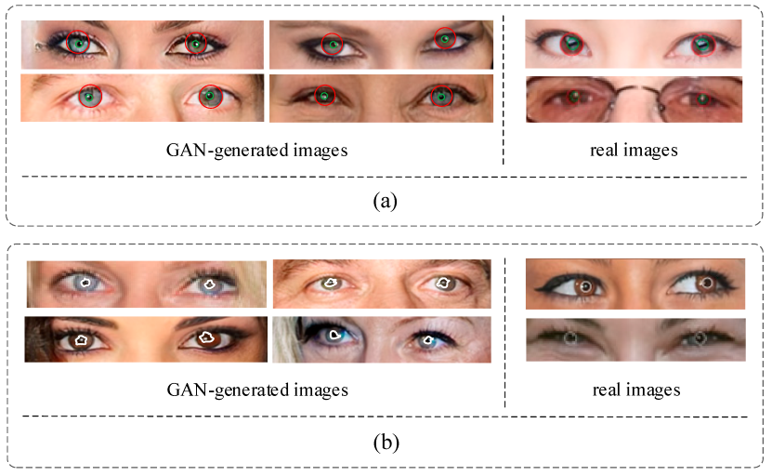
\includegraphics[width=5in]{img/pupil.png}
    \caption{\textit{Iris Color and Pupil Boundary}}
\end{figure}


\subsubsection{Residual Comparison}

Residual comparison involves analyzing the residuals obtained from subtracting the original image from its manipulated counterpart. By comparing the residuals, artifacts and inconsistencies introduced during the manipulation process can be detected. Unusual patterns or significant deviations between residuals may signify the presence of a deepfake.
\begin{figure}[htbp]
    \centering
    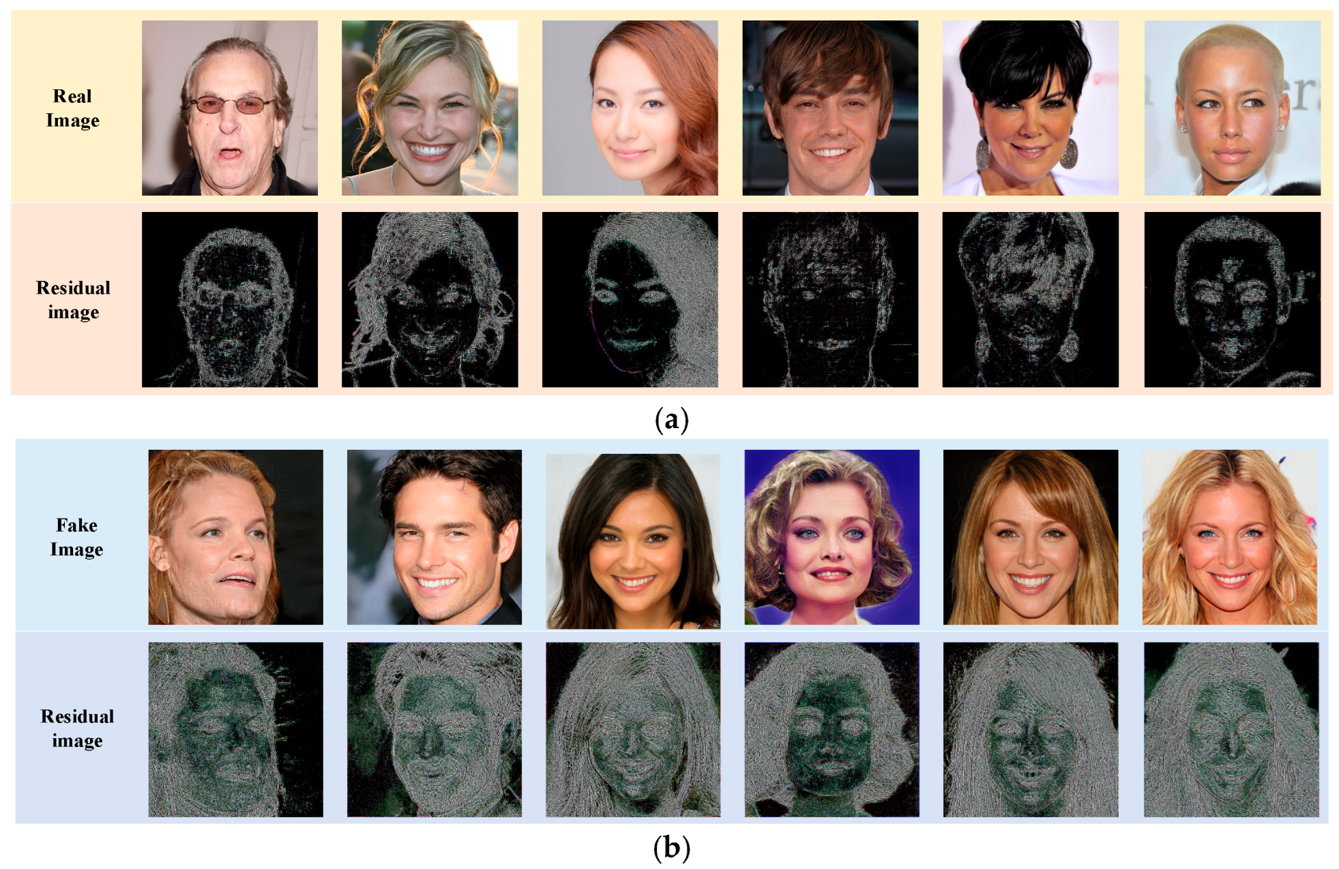
\includegraphics[width=5in]{img/residual.png}
    \caption{\textit{Residual Comparison}}
\end{figure}


\subsubsection{Kernel Density Estimation (KDE) of Color}

Kernel Density Estimation (KDE) involves estimating the probability density function of color values in an image. By applying KDE to different regions of an image, it becomes possible to identify unusual color distributions introduced by deepfake manipulation. Sudden spikes or dips in color density can be indicative of tampering.

\begin{figure}[htbp]
    \centering
    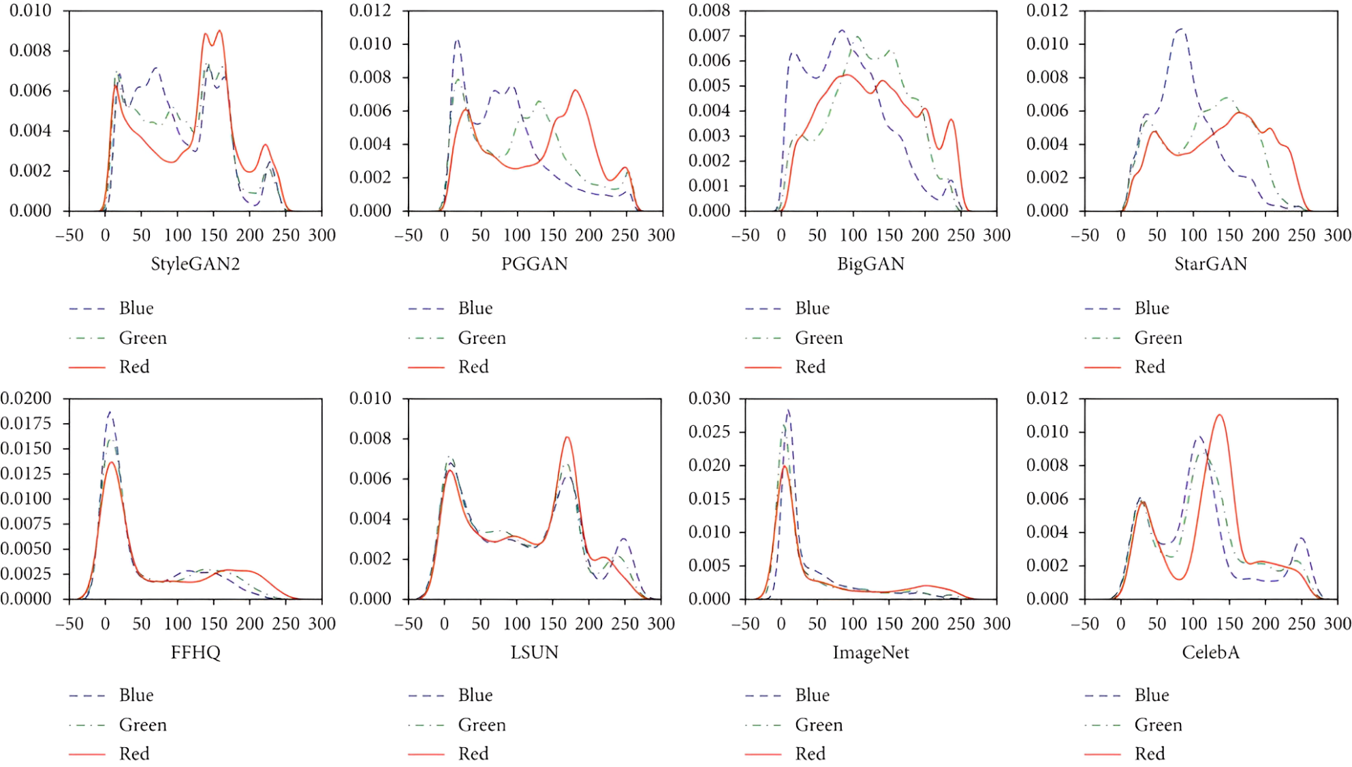
\includegraphics[width=5in]{img/KDE.png}
    \caption{\textit{Kernel Density Estimation (KDE) of Color}}
\end{figure}
